\graphicspath{ {./JiaweiZhuang/img/} }

\subsection{Basic behavior of blood and drug fields}

We first describe the basic behavior of blood and drug fields during the simulation. The $Re=5, Pe=1$ case is used as the major example, as the different cases show similar overall behavior (just with different magnitudes and diffusion rates). The effect of $Re$ and $Pe$ is discussed in the next section.

Because the x and y directions are symmetric in our problem, we can visualize the 3-D blood vessel using 2-D "longitudinal cuts", by slicing over the middle point of x-axis and only plot the y-z cross section. 

Fig \ref{fig:density} shows the blood density. The density oscillate according two the heart beat (please refer to the animation in the slides). Here we only plot two steps with the middle and the highest value. Because of the inlet flow from the left, density is high on the left and low on the right. The major transition happens in the middle stenotic/narrow region, which shows large density gradient.

\begin{figure}[H]
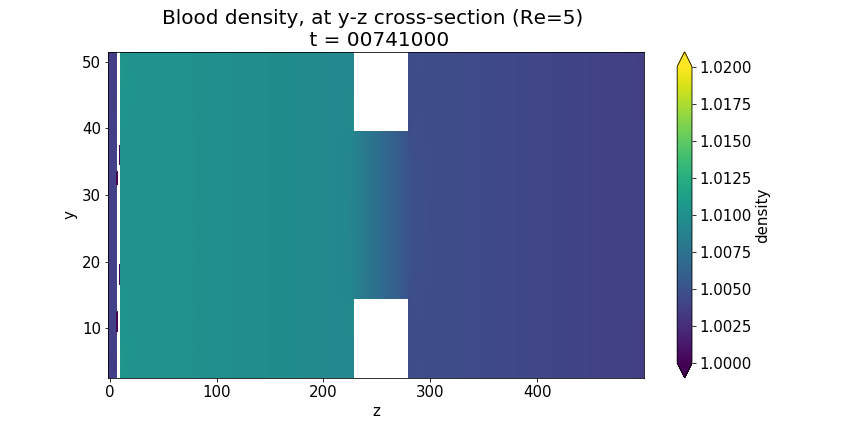
\includegraphics[scale=0.3]{cross_section/density_148}
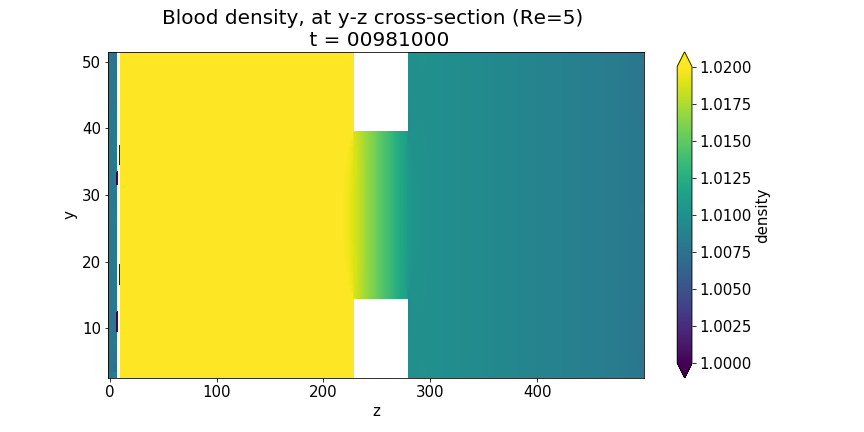
\includegraphics[scale=0.3]{cross_section/density_196}
\centering
\caption{Blood density at 2-D longitudinal cuts (Re=5, Pe=1 case).}
\label{fig:density}
\end{figure}

We then perform the Schlieren visualization on the density field, using the formula:

\begin{align}
Sch = exp(-k\frac{|\nabla T|}{max(|\nabla T|)})
\end{align}

where $T$ is the original field. Here it is the blood density.

Fig \ref{fig:sch} shows the Schlieren field with $k=20$. We don't see interesting patterns due to the lack of spatial gradient. Unlike Module 1’s Rayleigh-Benard Convection with highly complex patterns, in this blood flow case there is little spatial variations and the flows are highly laminar. The middle stenotic region has the highest Schlieren value, corresponding to the high gradient here.

\begin{figure}[H]
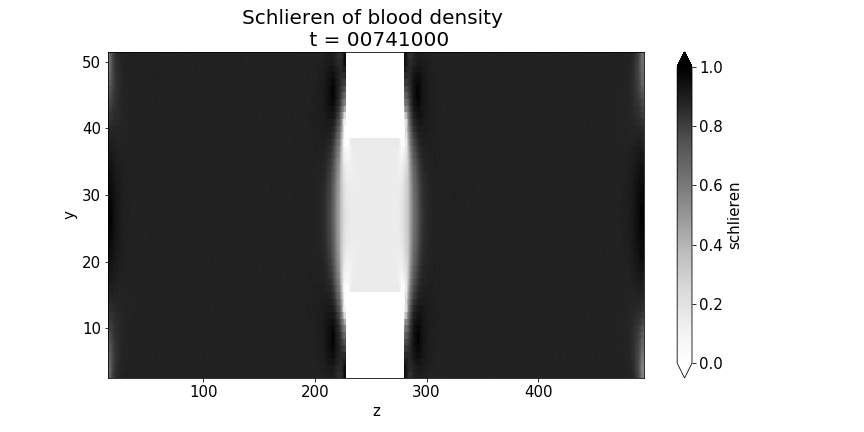
\includegraphics[scale=0.3]{cross_section/schlieren_148}
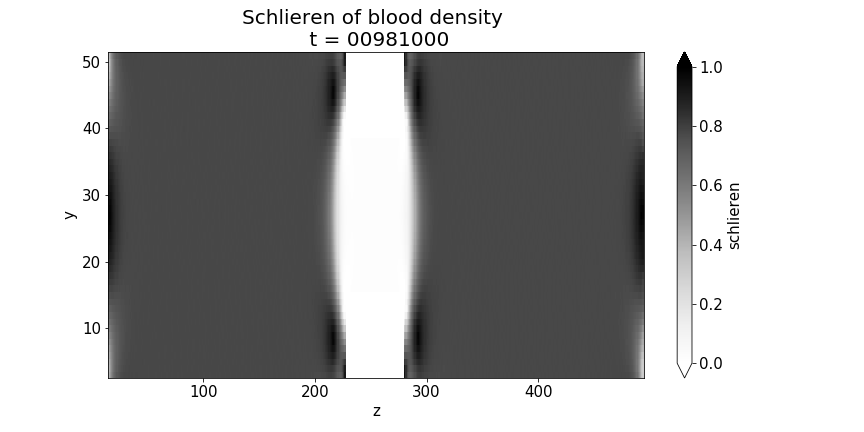
\includegraphics[scale=0.3]{cross_section/schlieren_196}
\centering
\caption{Schlieren visualization of blood density at 2-D longitudinal cuts (Re=5, Pe=1 case).}
\label{fig:sch}
\end{figure}

We then turn to the blood velocity. Fig \ref{fig:uz} shows the velocity magnitude and Fig \ref{fig:streamline} shows the streamline. Velocity also oscillates following the heart beat.
The stenotic region has the highest velocity, consistent with the continuity equation. The streamlines follow the the blood vessel shape.

\begin{figure}[H]
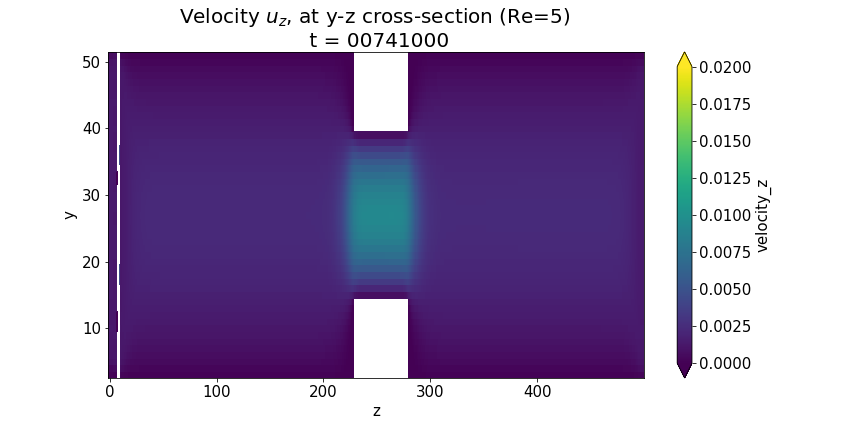
\includegraphics[scale=0.3]{cross_section/uz_148}
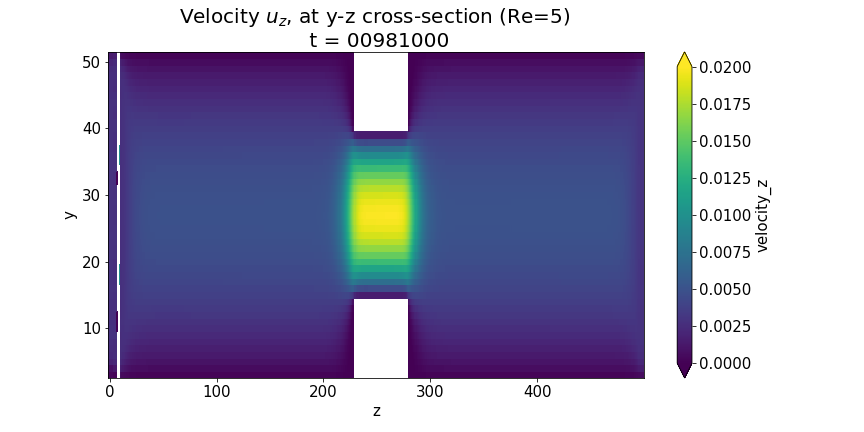
\includegraphics[scale=0.3]{cross_section/uz_196}
\centering
\caption{Blood velocity at 2-D longitudinal cuts (Re=5, Pe=1 case). Plotted is the z-component. The x, y components are orders of magnitude smaller and contribute little to the total magnitude.}
\label{fig:uz}
\end{figure}


\begin{figure}[H]
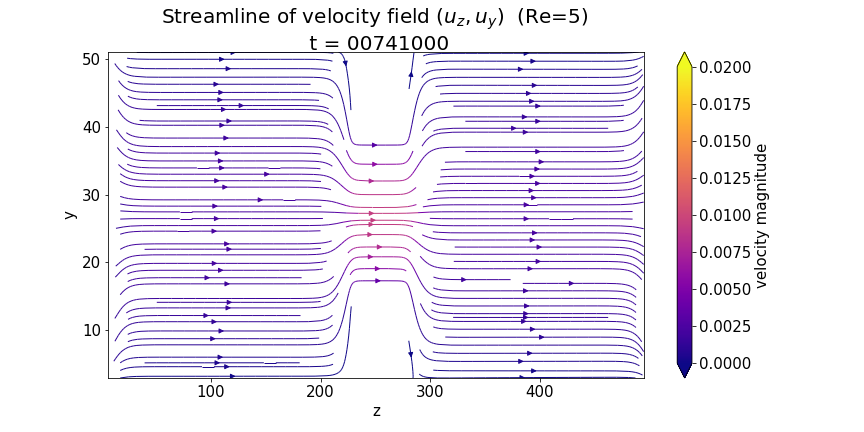
\includegraphics[scale=0.3]{cross_section/streamline_148}
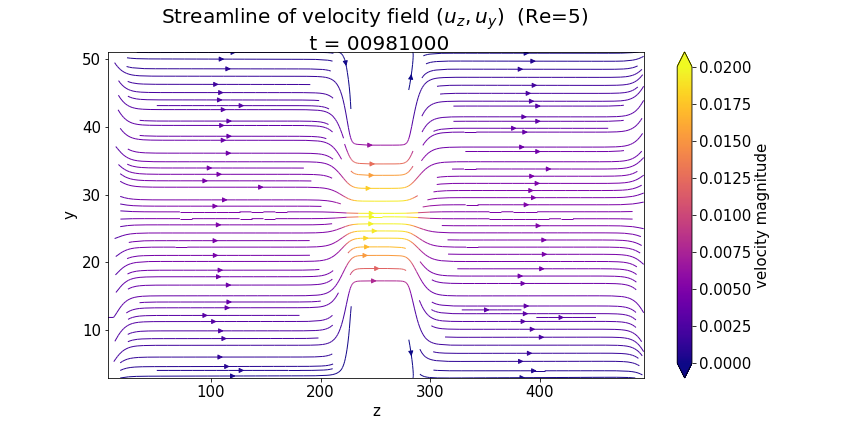
\includegraphics[scale=0.3]{cross_section/streamline_196}
\centering
\caption{Streamline of blood velocity at 2-D longitudinal cuts (Re=5, Pe=1 case), colorred with velocity magnitude.}
\label{fig:streamline}
\end{figure}

Last, we visualize the diffusion of the drug, in Fig \ref{fig:drug}. The drug is released at $1/4$ of total simulation time ($1 \times 10^6$ steps). It then gets diffused very quickly and pushed rightward following the flow direction. Just after 20,000 steps ($0.5\%$ of total simulation time), the main body of the drug field enters the stenotic region.

\begin{figure}[H]
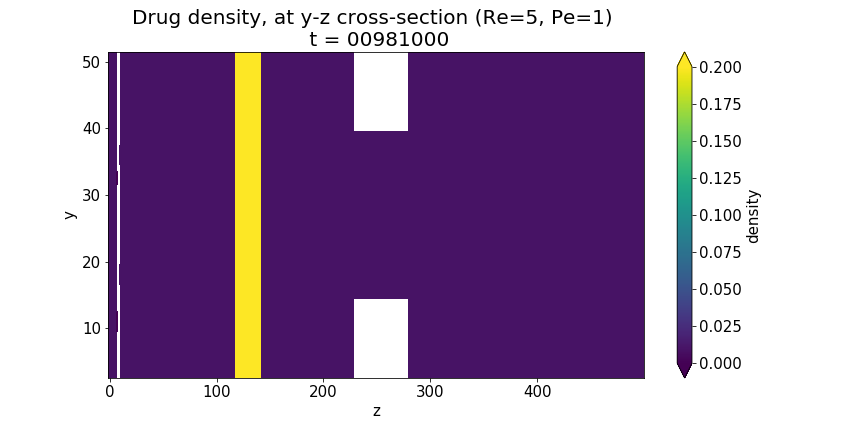
\includegraphics[scale=0.3]{cross_section/drug_196}
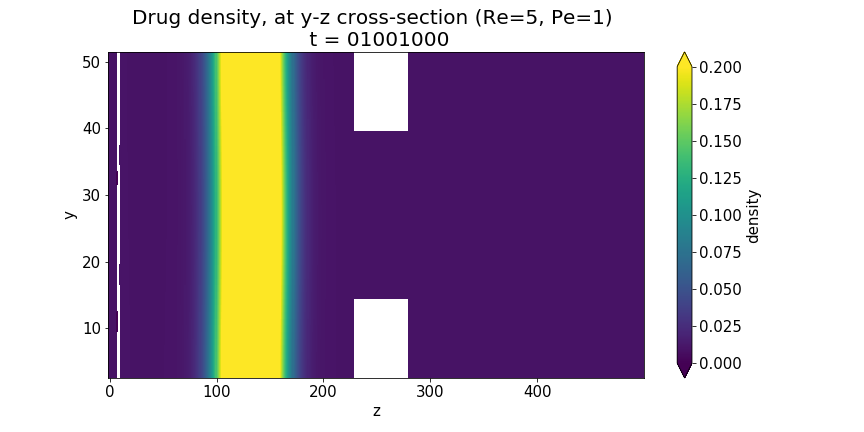
\includegraphics[scale=0.3]{cross_section/drug_200}
\centering
\phantomcaption
\end{figure}

\begin{figure}[H]\ContinuedFloat
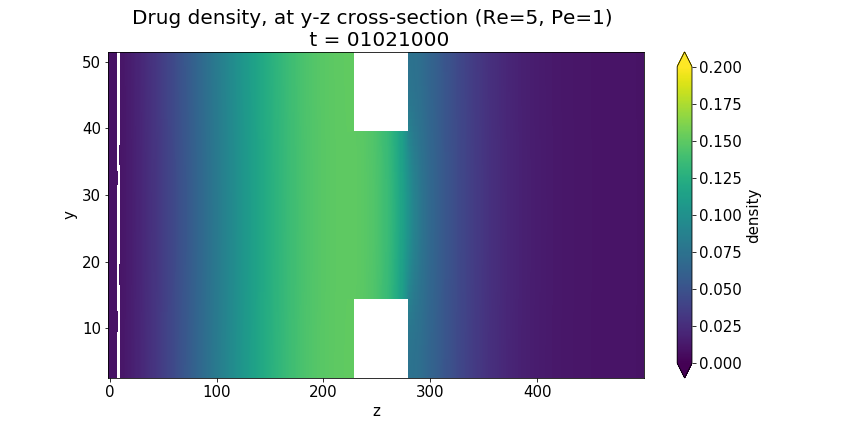
\includegraphics[scale=0.3]{cross_section/drug_204}
\centering
\caption{Drug density at 2-D longitudinal cuts (Re=5, Pe=1 case)}
\label{fig:drug}
\end{figure}

\subsection{Effect of Peclet number and Reynolds numbers on drug efficacy}

To better show the drug spread over time, we plot the drug profile averaged over the cross-section (x, y directions). Fig \ref{fig:drug_profile} shows the profiles for Re5Pe1 and Re5Pe3 cases. A larger Peclet number leads to slower diffusion of drug, as expected (due to higher viscosity). The profile has minor discontinuities at the entries of the stenotic region, due to the abrupt change in the denominator (cross-section size) when computing the mean.

\begin{figure}[H]\ContinuedFloat
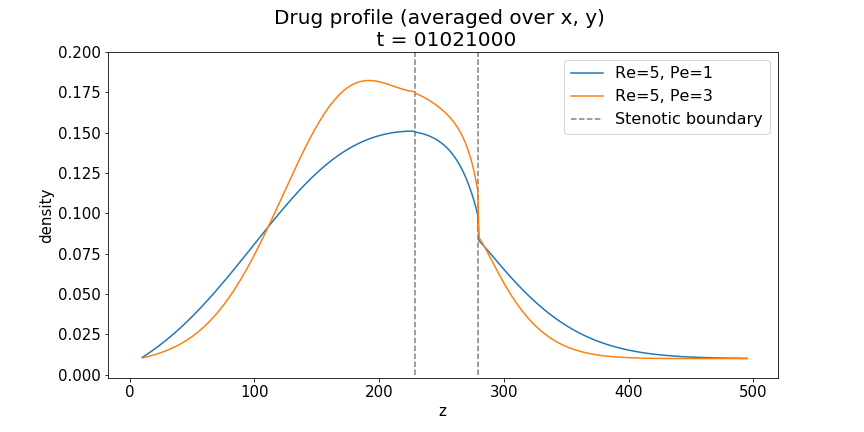
\includegraphics[scale=0.4]{drug_profile/drug_profile_204}
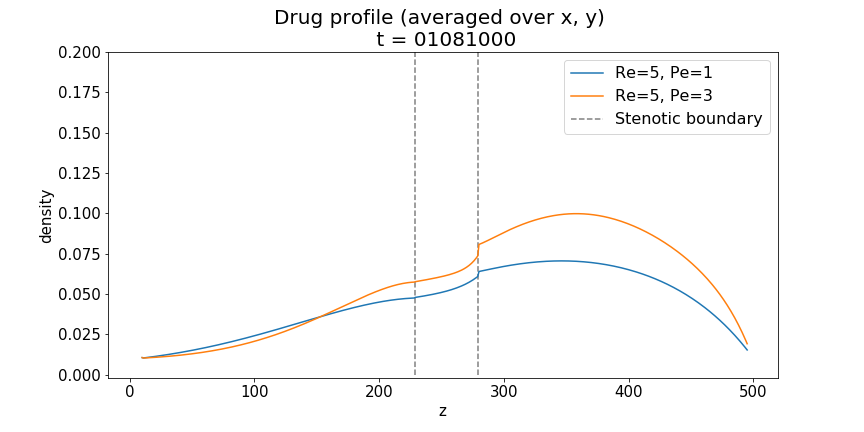
\includegraphics[scale=0.4]{drug_profile/drug_profile_216}
\centering
\caption{Drug profile averaged over x-y cross-section, for Re5Pe1 and Re5Pe3 cases.}
\label{fig:drug_profile}
\end{figure}

To show the drug efficacy, we compute the integral of drug density (i.e. drug mass) over the stenotic region, as plotted in Fig \ref{fig:drug_efficacy}. After the drug lease at $step = 1 \times 10^6$, it diffuses very quickly, in less than $5 \times 10^5$ steps ($1/8$ of the total time). Again, a large Peclet number leads to slower diffusion and thus higher drug efficacy. For the large Reynold number case (Re10), the drug mass is 8 times higher, proportional to the increased domain size; but the time evolution has a similar trend as Re5 cases.

\begin{figure}[H]
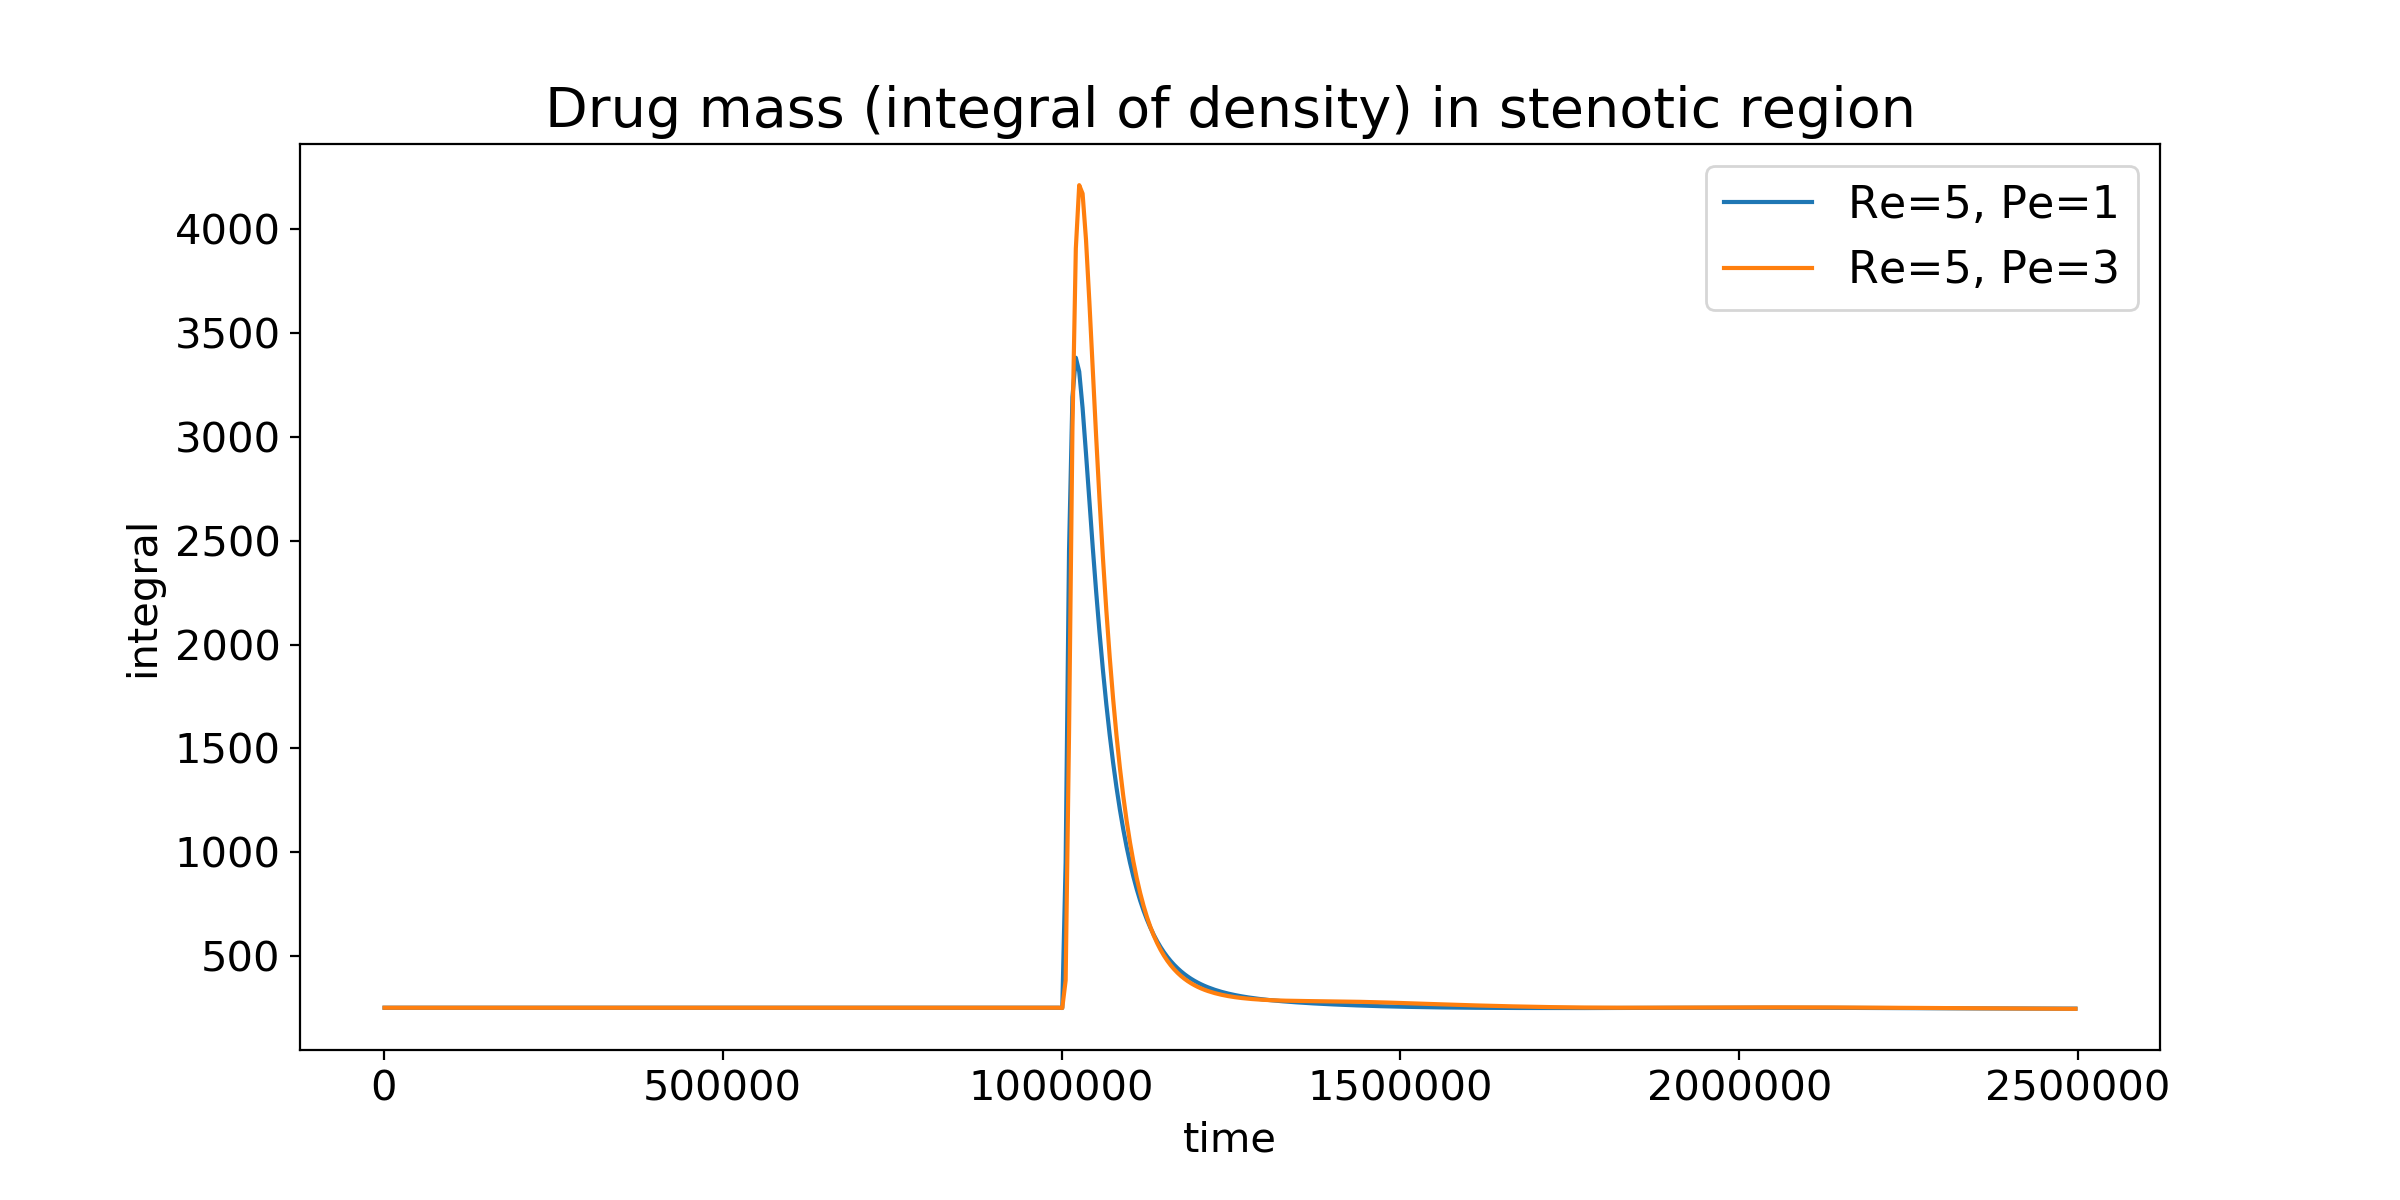
\includegraphics[scale=0.4]{drug_efficacy/drug_integral_re5_fulltime.png}
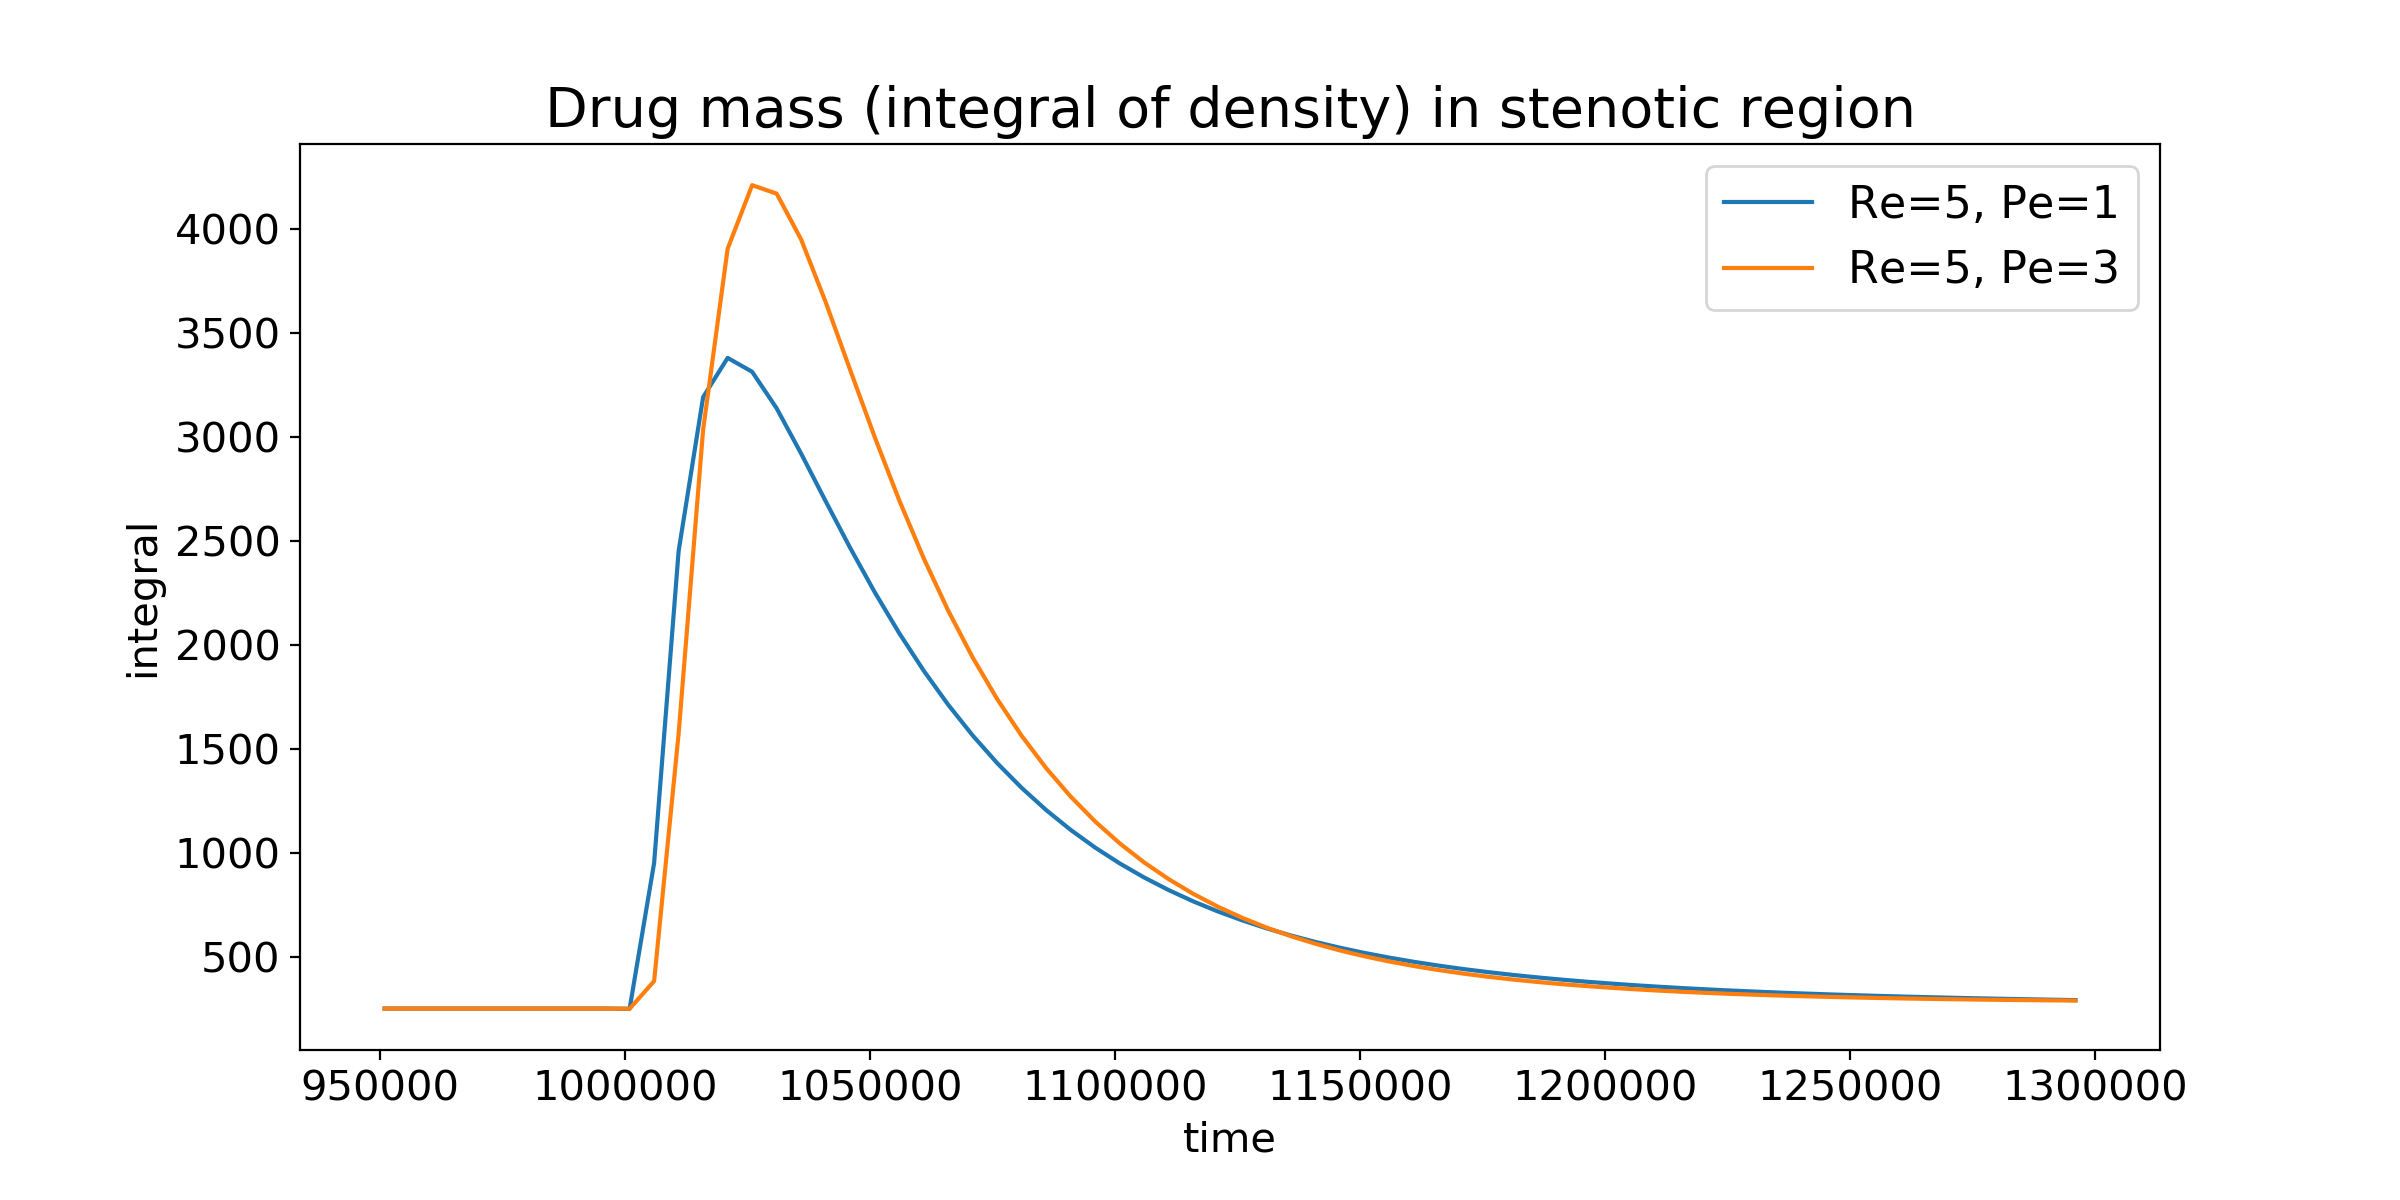
\includegraphics[scale=0.4]{drug_efficacy/drug_integral_re5_hightime.png}
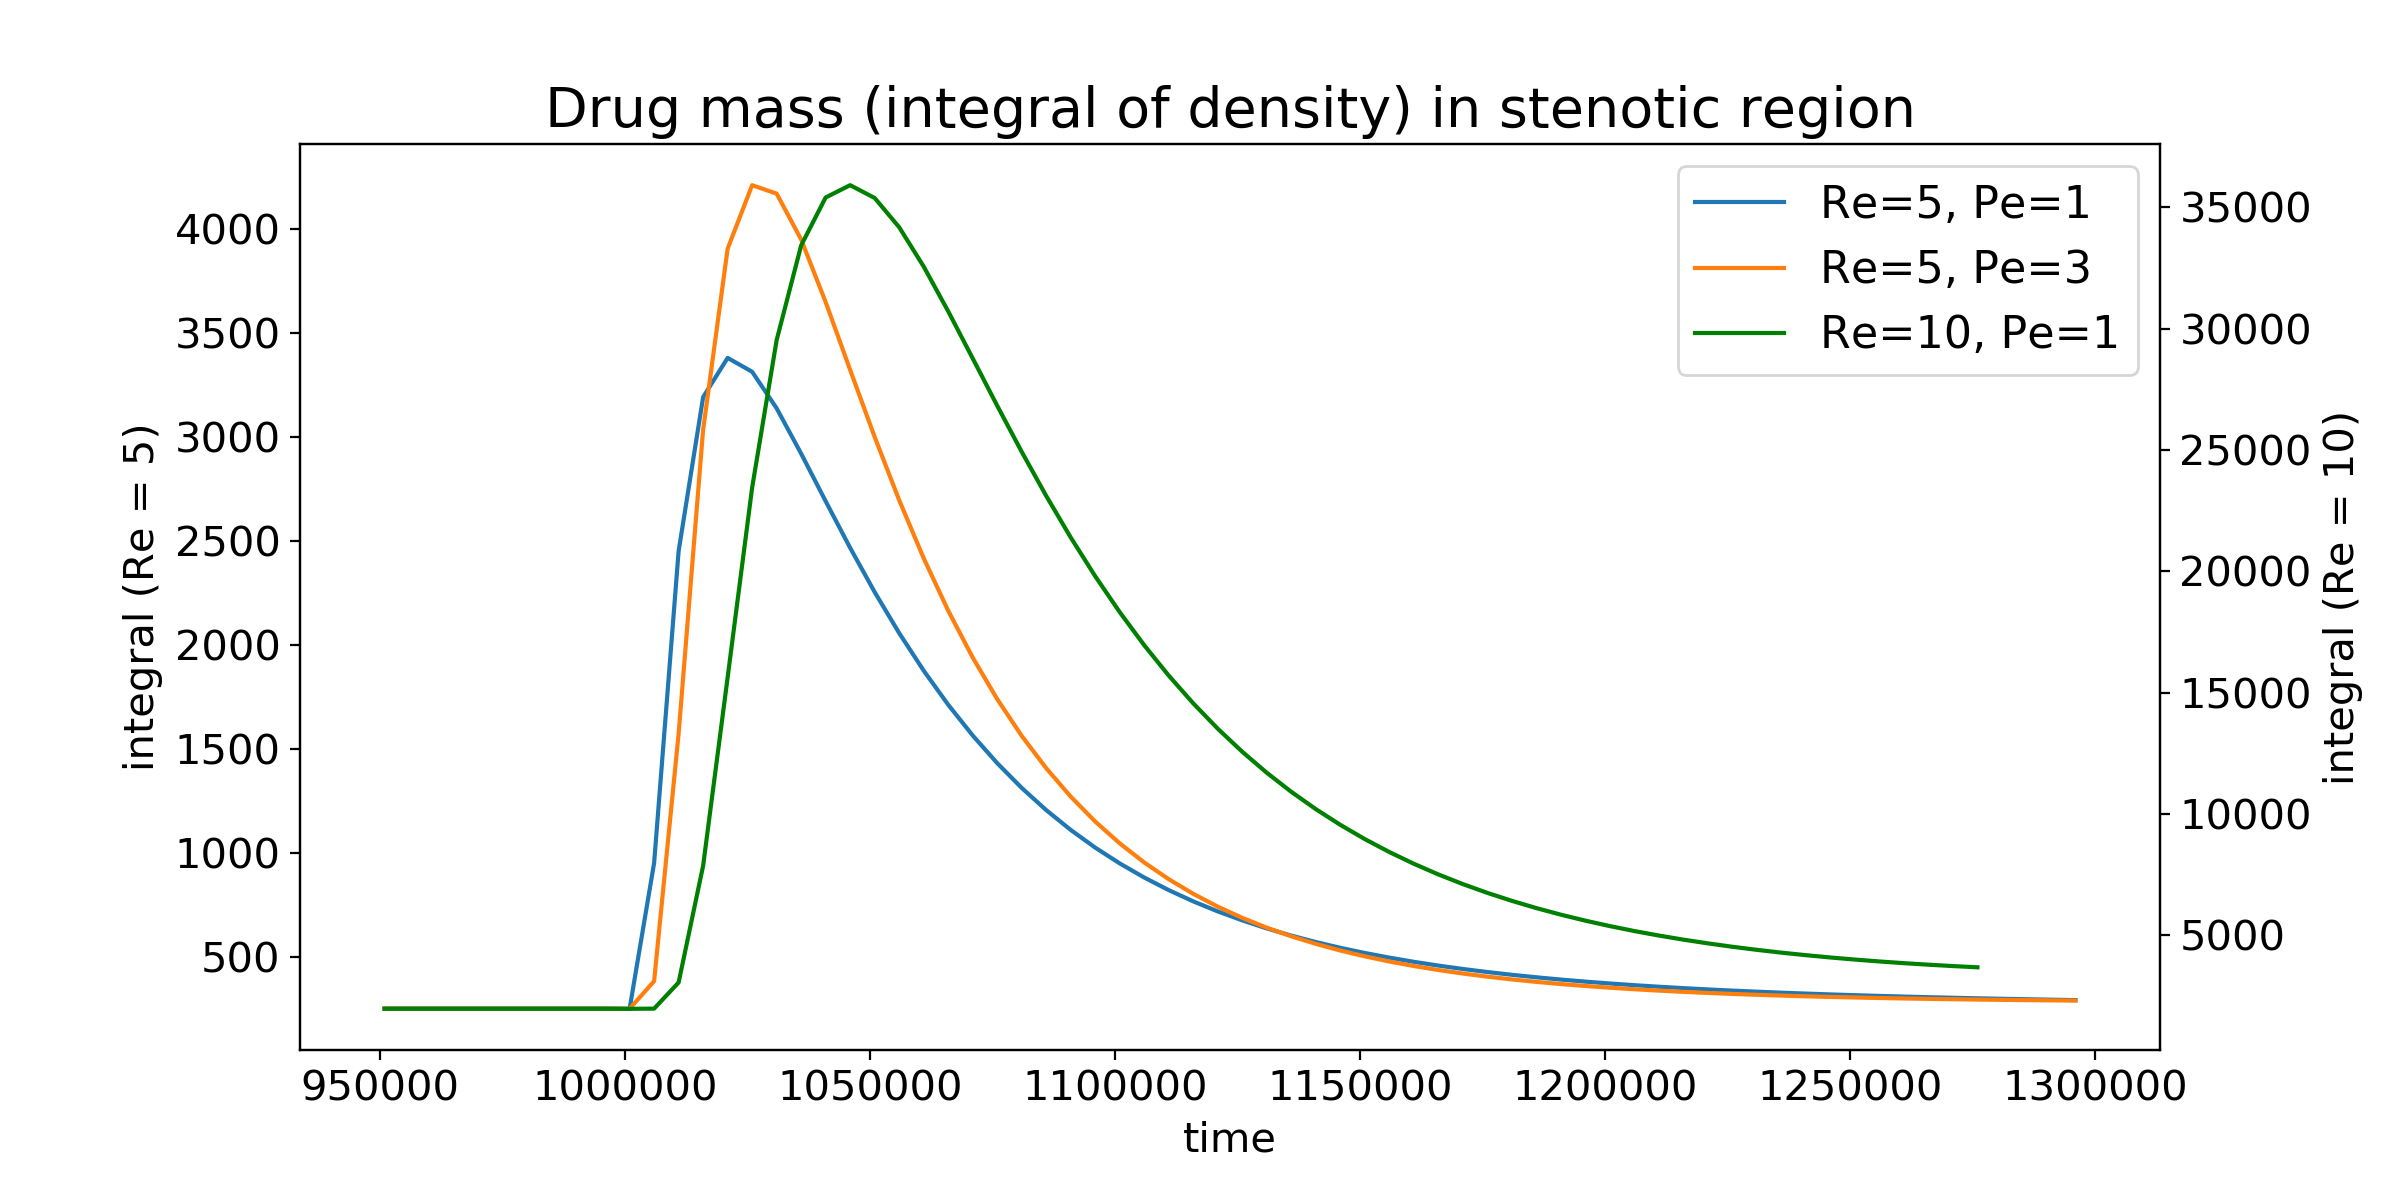
\includegraphics[scale=0.4]{drug_efficacy/drug_integral_re5and10_hightime.png}
\centering
\caption{Drug efficacy (integral over narrow region. The first figure shows the full time axis. The second figure is the zoomed-in version, highlighting the period with high drug density. The third figures adds the Re10 case on a twin y-axis.}
\label{fig:drug_efficacy}
\end{figure}

\subsection{3-D streamline visualization}

A particularly interesting phenomenon can be shown in 3D streamline visualization. We use ParaView StreamTracer to visualize the blood streamline at a single time slice, as shown in Fig \ref{fig:streamline_demo}. Different time slices have similar streamlines although different velocity magnitudes. Near the entries of the stenotic region, there are many small whirls, forming a big circle.

\begin{figure}[H]
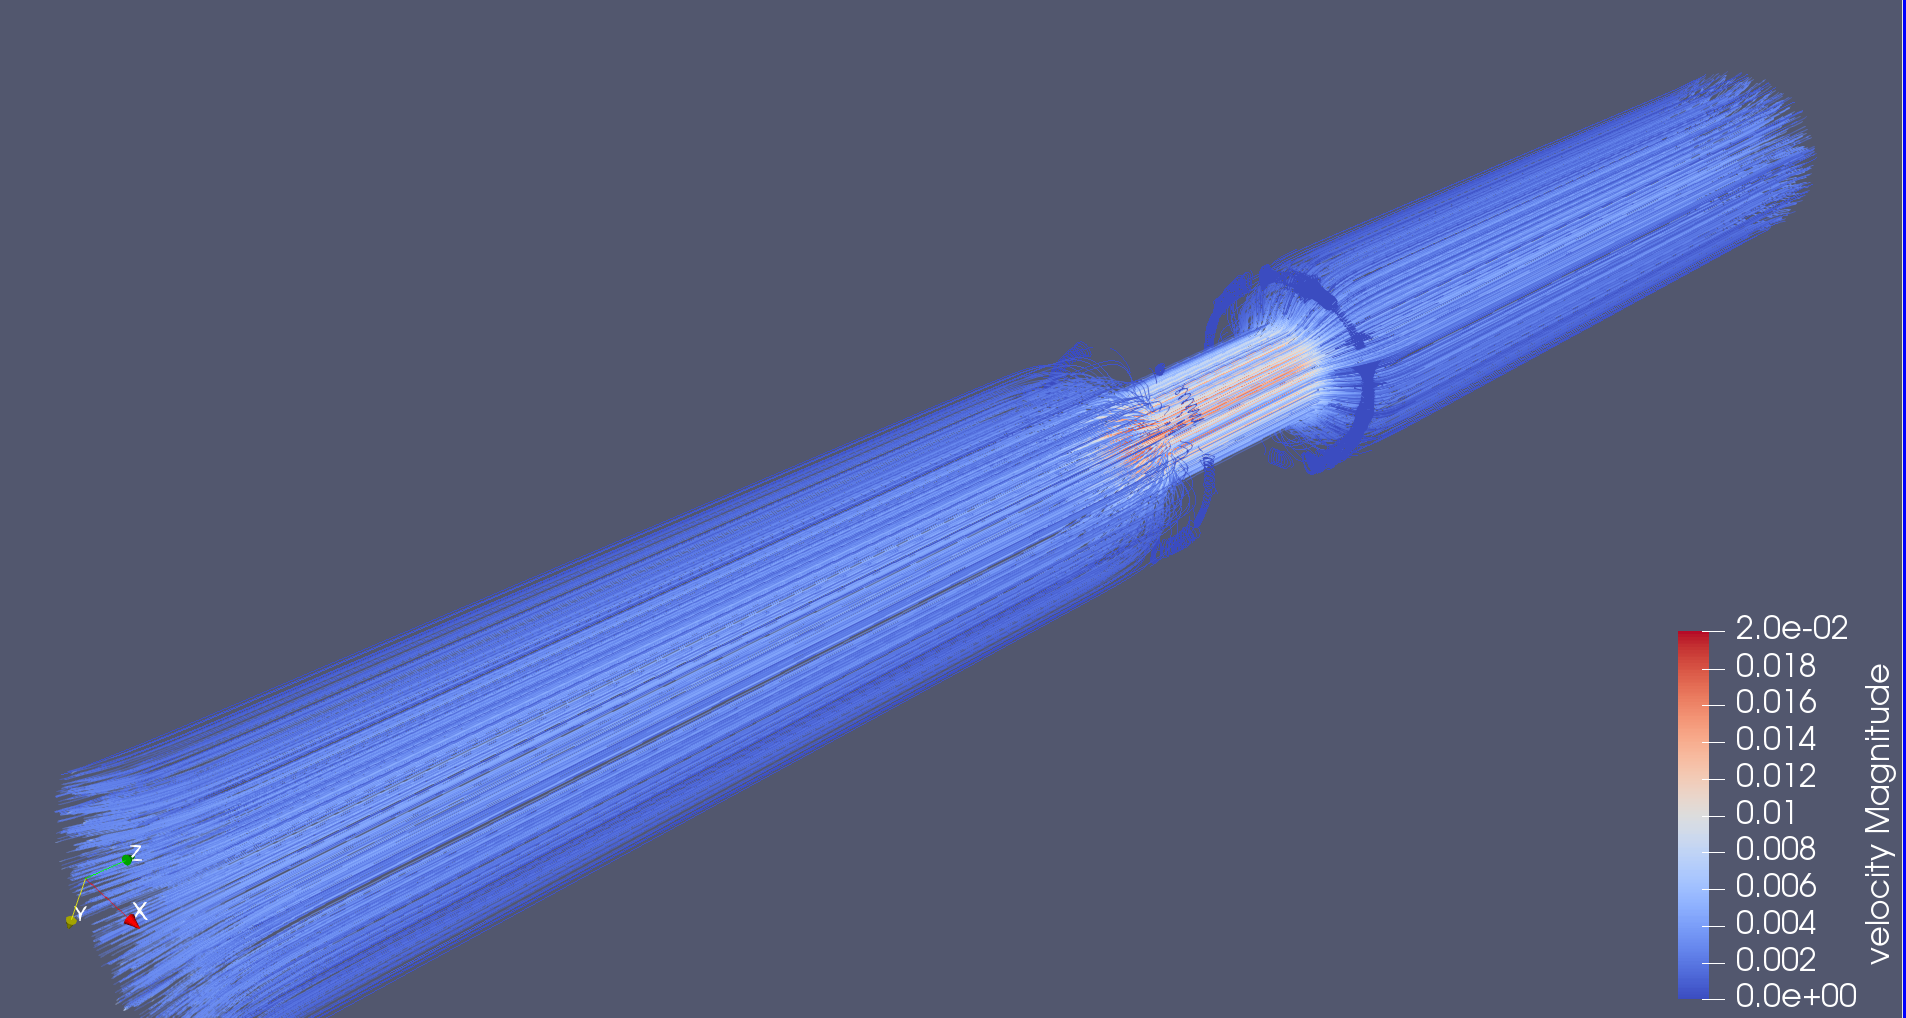
\includegraphics[scale=0.44]{streamline_3d/streamline_demo.png}
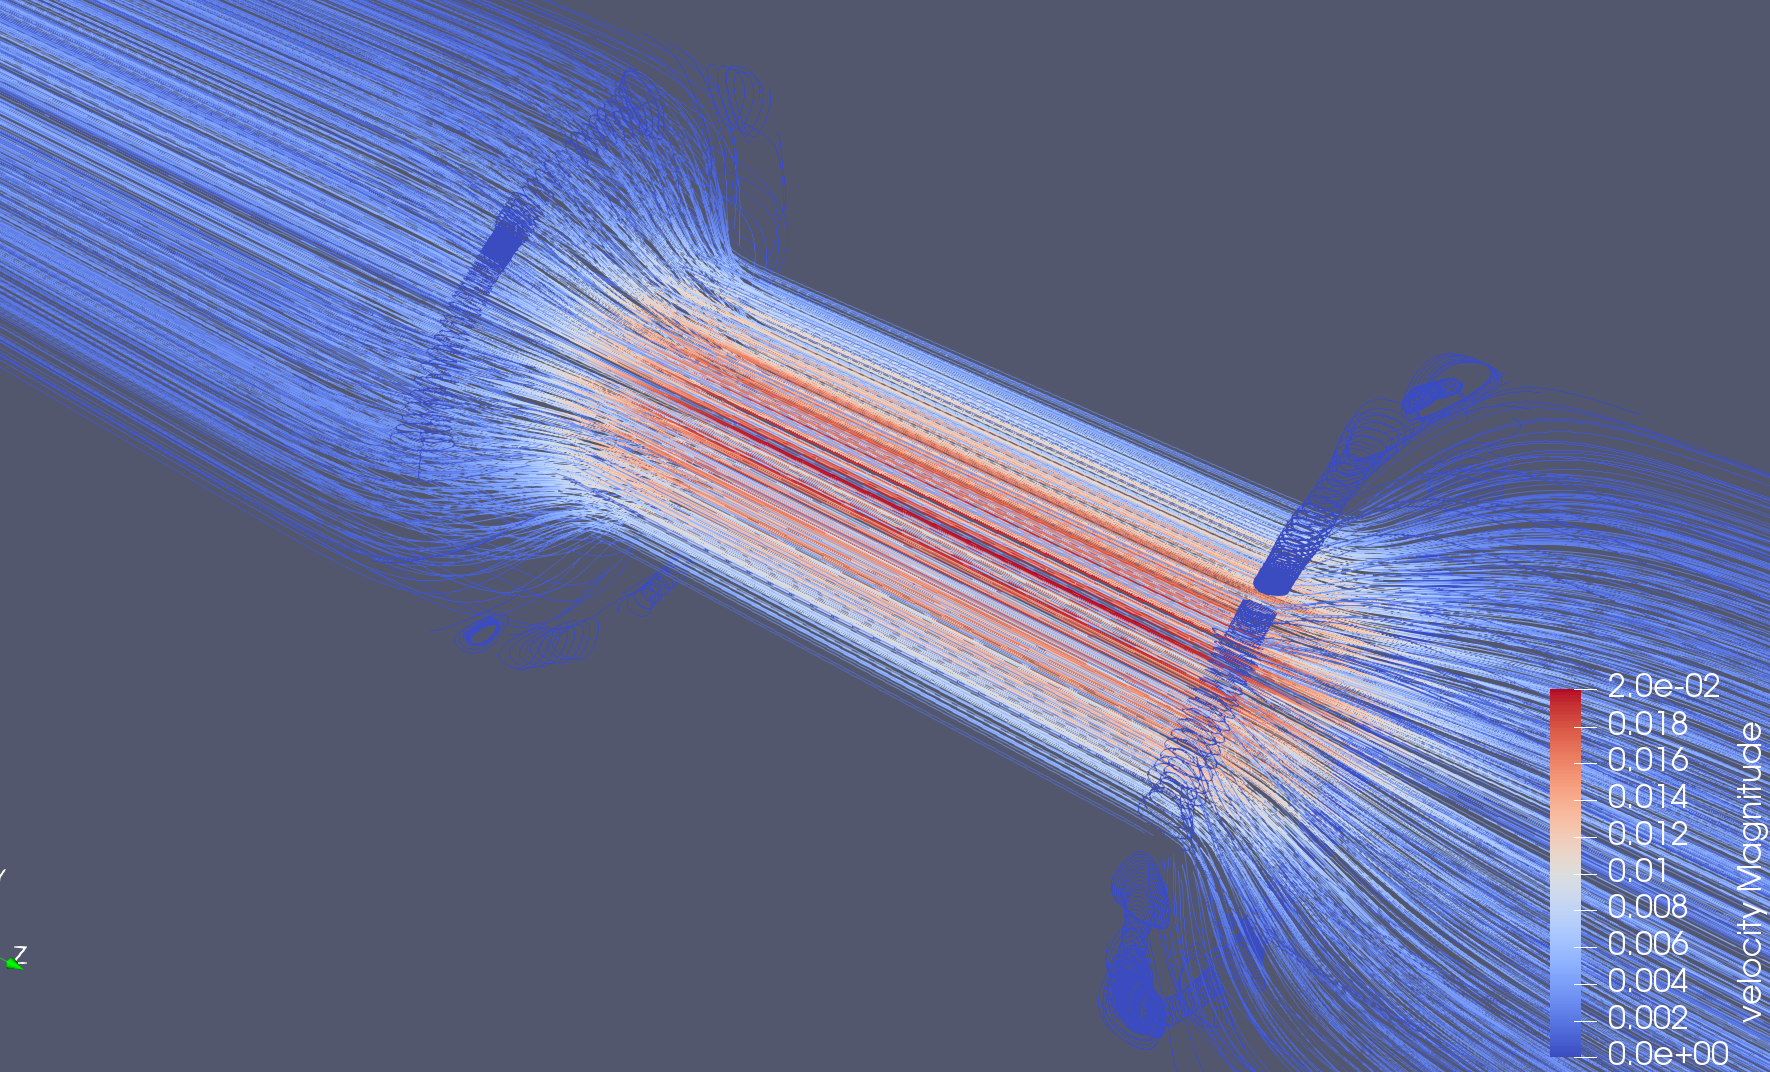
\includegraphics[scale=0.48]{streamline_3d/small_whirls_demo.png}
\caption{3-D Streamlines generated by ParaView. Colors are velocity magnitudes.}
\label{fig:streamline_demo}
\end{figure}

To further highlight to streamline, we color the lines with streamline types \footnote{https://kitware.github.io/paraview-docs/latest/python/paraview.simple.StreamTracer.html} instead of velocity magnitude, as shown in Fig \ref{fig:streamline_color}. A value of 1 (blue color) means that the streamline exceeds the domain boundary. Most streamlines belong to this case, as they all go from the left inlet to the right outlet. A value of 3 or more (white or red colors) means that streamline terminates due to the violation of some limits such as line length or integration steps. The small whirls belong to this case as they form a closed circle without connecting to external boundaries. Those small whirls occur when the fluid hit the blood vessel boundary and bounce back. 

\begin{figure}[H]
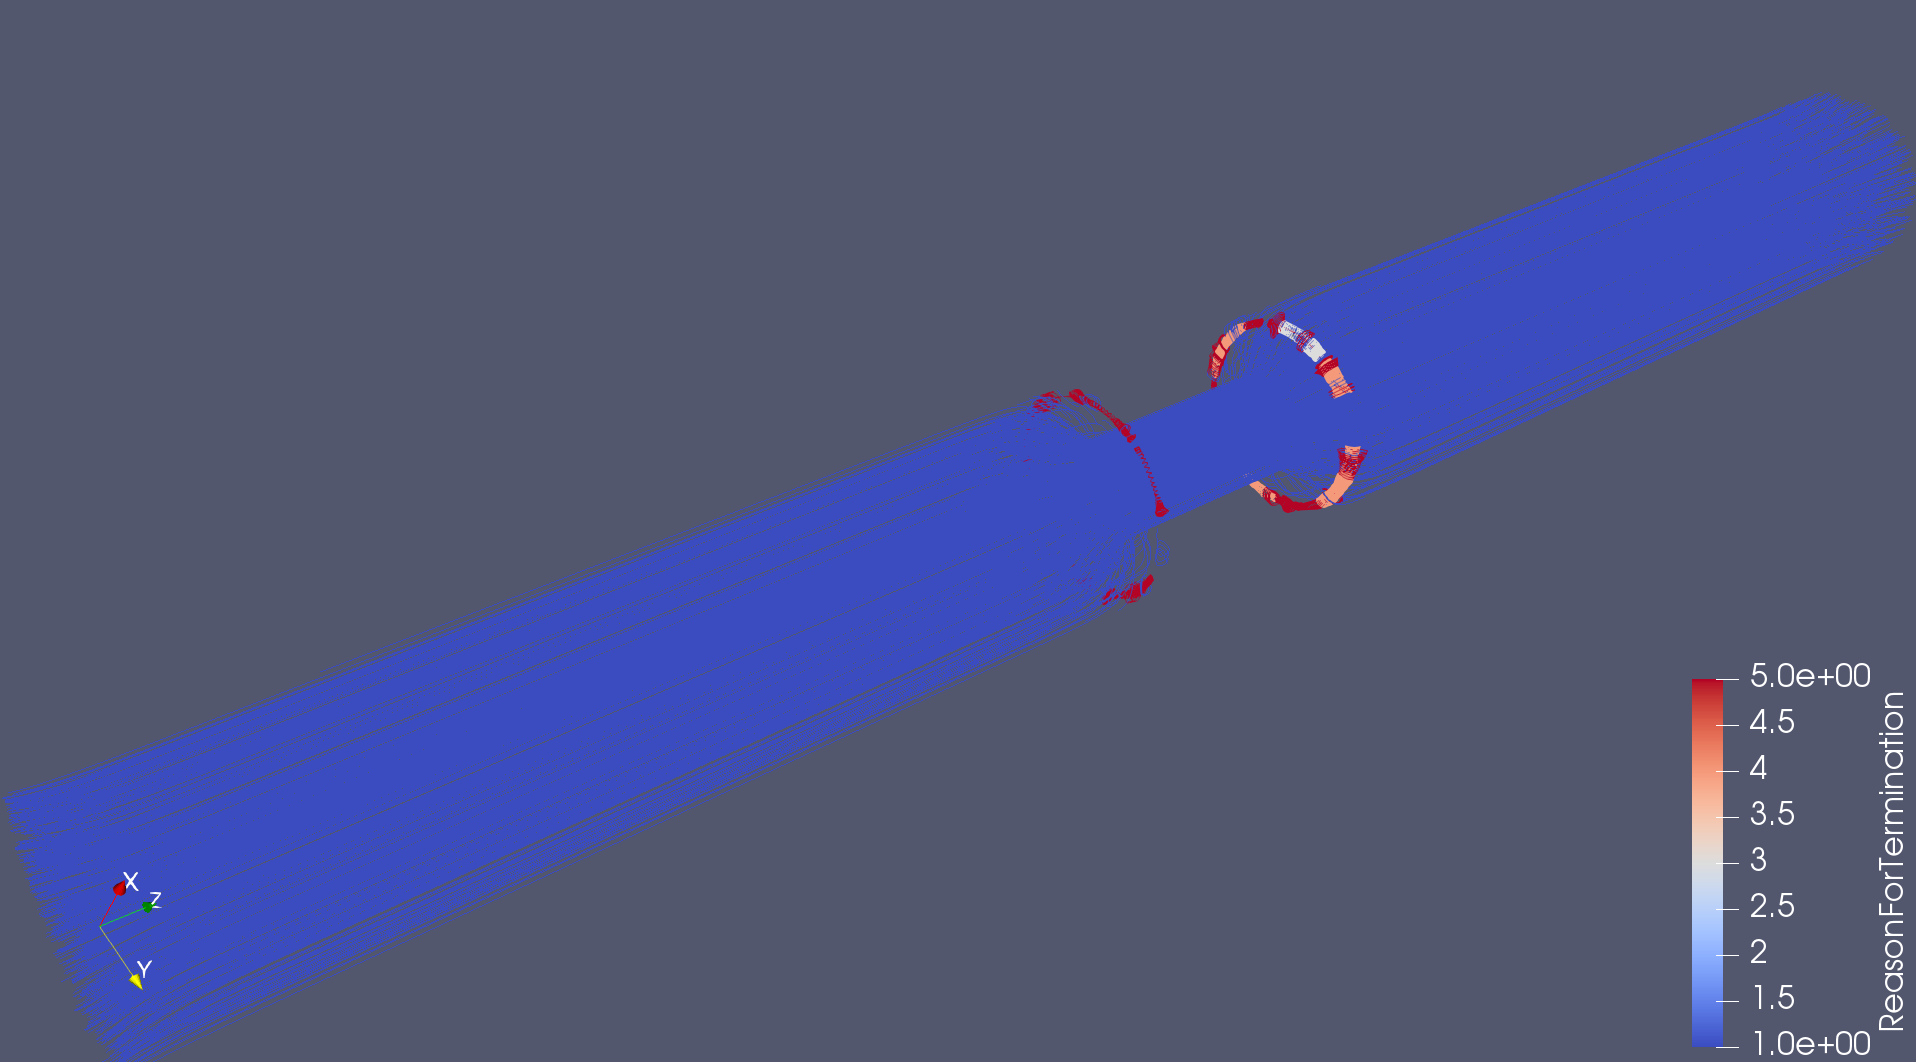
\includegraphics[scale=0.45]{streamline_3d/streamline_color.png}
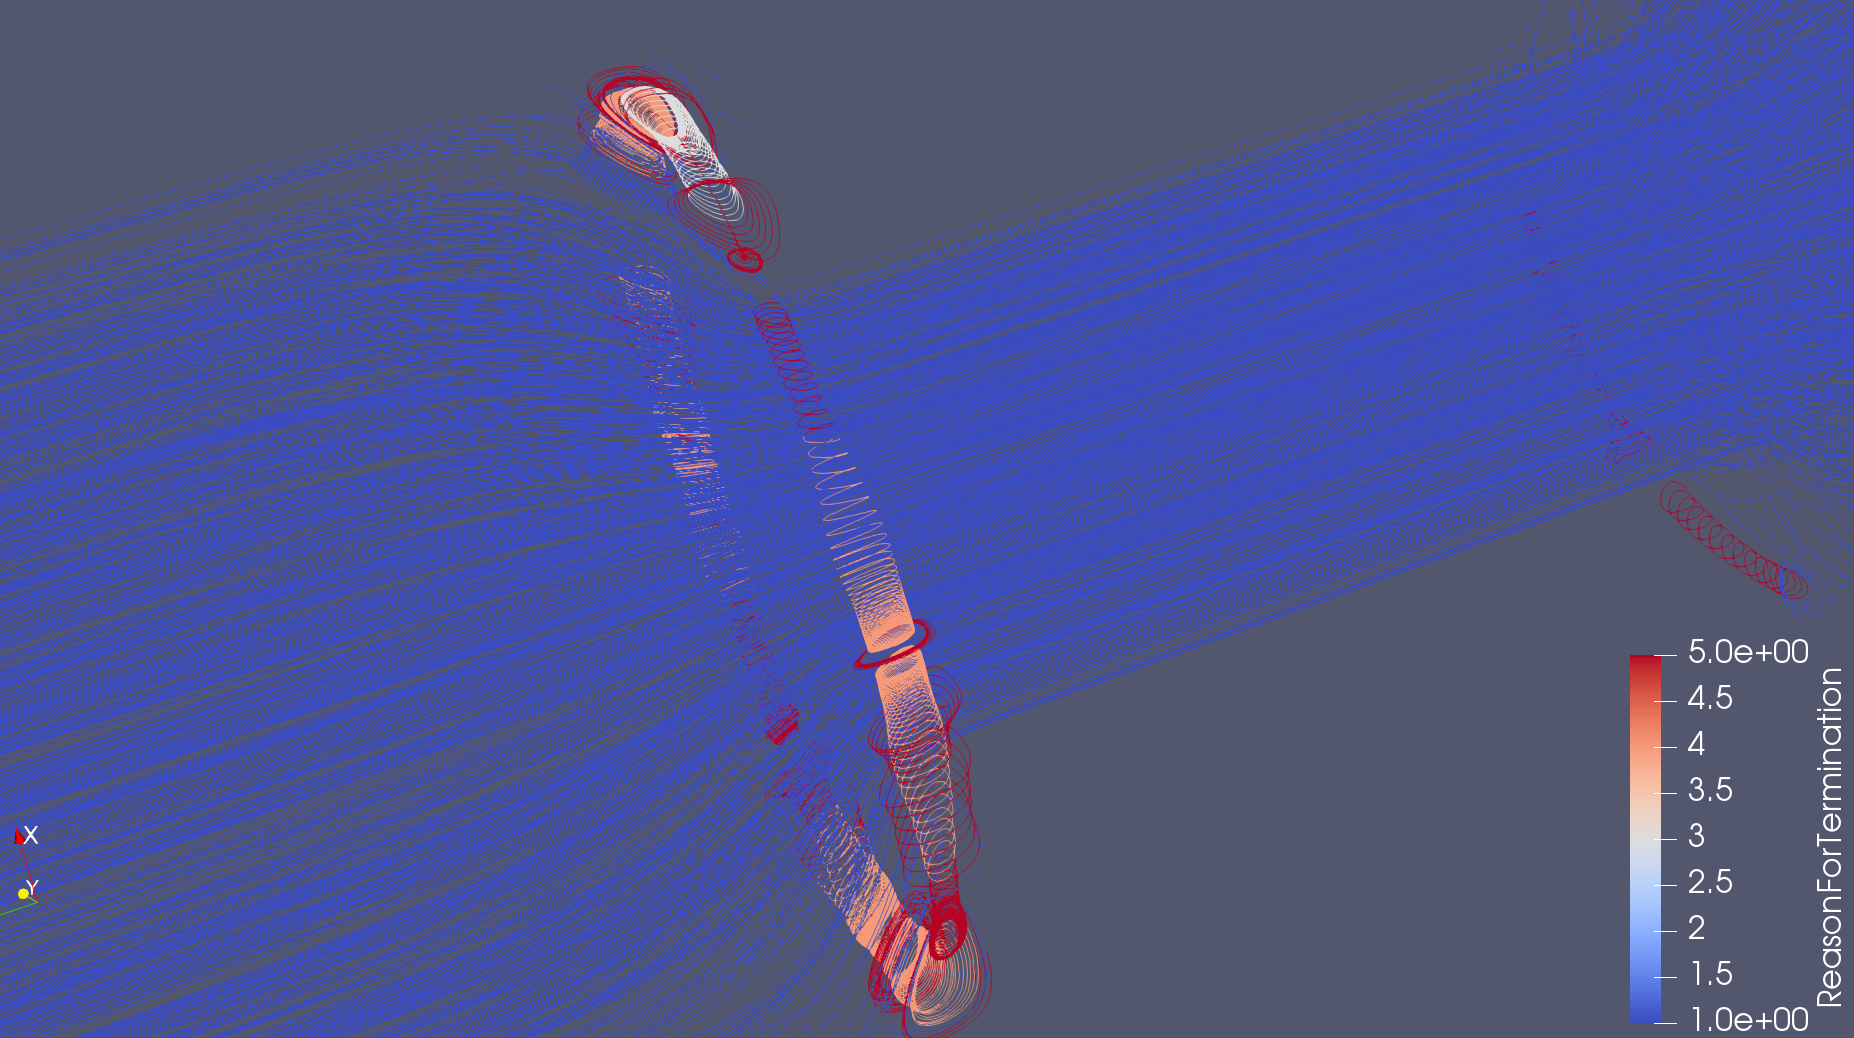
\includegraphics[scale=0.47]{streamline_3d/small_whirls_color.png}
\caption{3-D Streamlines generated by ParaView. Colors are streamline types, to highlight the small whirls.}
\label{fig:streamline_color}
\end{figure}

\subsection{Data post-processing methods and code availability}

The original VTK files generated by Murphy simulations are very big and difficult to analyze. The output frequency is set to every $1000$ steps; with the total $4 \times 10^6$ steps, 4000 output files are generated for each simulation case.

\begin{itemize}
	\item For $Re = 5$ cases, each time step produces $224 MB$ data, leading to $224 MB \times 4000 = 900 GB$ total data.
	\item For $Re = 10$ cases, each time step produces $1753 MB$ data, leading to $1753 MB \times 4000 = 7000 GB$ total data.
\end{itemize}

The file size calculation is available at: JiaweiZhuang/check\_raw\_vtk\_files.ipynb

Considering a typical disk throughput of 500 MB/s, reading 1000 GB data will take 30 minutes. Analyzing such huge data in the real-time is not feasible. 

To efficiently process and visualize the data, we conducted the following steps:

\begin{itemize}
	\item \textbf{Down-sampling}. Because the physical system is changing slowly, with a time scale determined by the heart beat frequency, the original 1000-step output frequency is not necessary. We can still resolve the flow evolution with a 5000-step frequency. This reduces the data size by 5 times.
	\item \textbf{Reorganizing and compressing}. Although our problem is defined on a 3D uniform grid mesh, the VTK files store the data as unstructured meshes. The grid coordinates are unnecessarily repeated for each grid point. By storing the same data as structured 3-D arrays, we removed the redundant grid coordinate information. The 3-D data are then written to NetCDF format, with additional compression. We use vtki (https://github.com/vtkiorg/vtki) to load VTK files in Python, and then use Xarray (https://github.com/pydata/xarray) to write and read NetCDF files. The scripts for this step are JiaweiZhuang/preprocess\_vtk.py and JiaweiZhuang/submit\_preprocess.sh. This step further reduces data size by 10 times. 
	\item \textbf{Out-of-core computing}. Although the final data size is reduced to about 100 GB, it is still much bigger than the CPU memory of a normal laptop, and close to the total memory of a compute node on Odyssey cluster. We use Dask (https://github.com/dask/dask) for out-of-core computation to avoid exhausting the memory. The code for this step is JiaweiZhuang/all\_plots\_for\_report.ipynb
\end{itemize}

Those post-processing optimizations allow us to generate the plots for this report and the presentation in a few hours, instead of many days.